\subsection{Resumo}

\begin{table}[h!]
\centering
\begin{tabular}{ |c|c|c|c|c|  }
\hline
\rowcolor{lightgray}
Algoritmo & Max & Min & Média & Desvio Padrão \\
\hline
Hill-Climbing & 2.369 & 0.144 & 1.05 & 0.682 \\
\hline
Hill-Climbing com restart & 2.556 & 0.0 & 1.137 & 0.795 \\
\hline
Simulated Annealing & 3.089 & 0.546 & 1.48 & 0.711 \\
\hline
Genetic Algorithm & 1.949 & 0.037 & 1.027 & 0.737 \\
\hline

\end{tabular}
\caption{Tabela com dados consolidados dos algoritmos}
\end{table}

\begin{figure}[H]
\centering
  \begin{minipage}[b]{0.48\textwidth}
    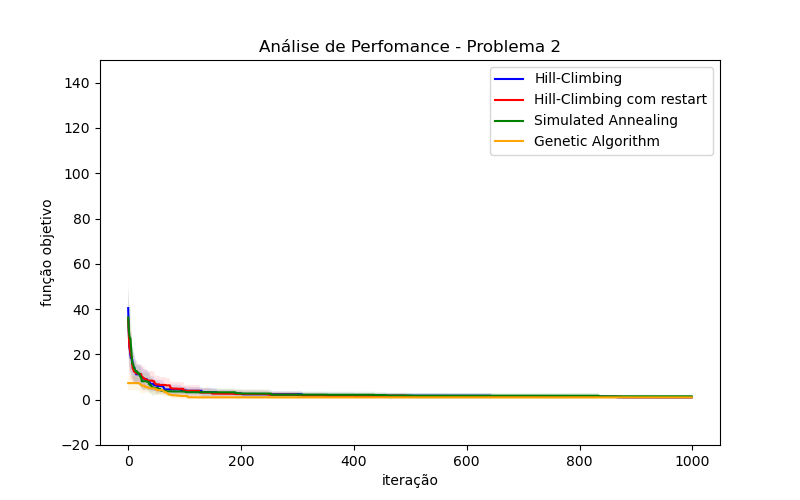
\includegraphics[width=88mm]{imagens/otima/problema-2-performance-algoritmos-best.png}
    \caption{Dados da execução da função objetivo durante as 10 iterações por melhor valor.
    \label{fig:problema-2-performance-algoritmos-best}}
  \end{minipage}
  \hfill
  \begin{minipage}[b]{0.48\textwidth}
    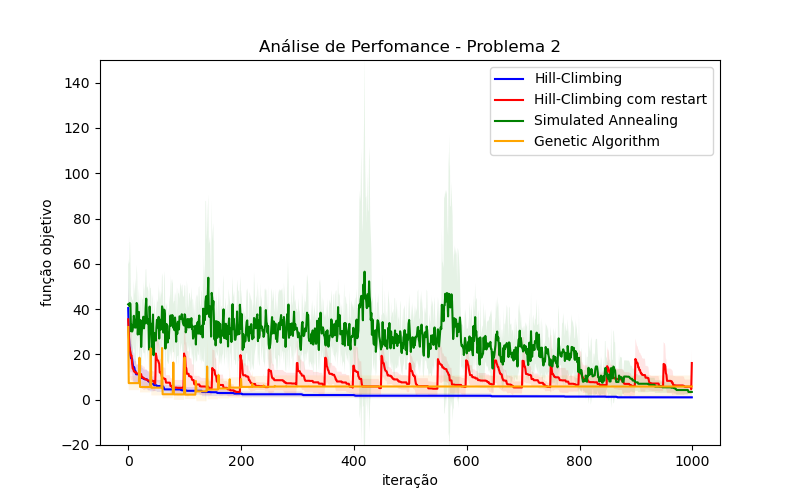
\includegraphics[width=88mm]{imagens/otima/problema-2-performance-algoritmos-value.png}
    \caption{Dados da execução da função objetivo durante as 10 iterações por valor atual.
    \label{fig:problema-2-performance-algoritmos-value}}
  \end{minipage}
\end{figure}